%! Author = Gianni
%! Date = 08/02/2024

\chapter{Flask web server}
\label{ch:flask-web-server}

\section{Implementazione nel progetto}
\label{sec:flask-introduzione}
Flask è un framework web scritto in Python per la creazione di siti e interfacce web
ed è una applicazione WSGI (Web Server Gateway Interface).
Viene considerato un micro-framework perché ha un nucleo semplice e minimale, 
ma è estendibile con librerie di terze parti.
In questo modo si possono aggiungere le funzionalità comuni presenti in altri framework più complessi.
La sua modularità fa sì che possa essere impiegato sia da principianti che da professionisti.
In questo progetto Flask è stato usato per l'esecuzione di script python da browser per facilitare
la generazione dei modelli utili per la virtualizzazione di sensori e modelli di crescita.
Di seguito viene spiegato come funziona il framework e come è stata strutturata l'applicazione web.

\section{Installazione}
\label{sec:flask-installazione}
L'installazione può essere eseguita su qualsiasi sistema operativo in cui può essere installato Python.
Nella guida ufficiale \cite{flask-doc} viene specificato 
che la versione 3 di Flask è compatibile con Python a partire dalla versione 3.8, 
tuttavia è possibile usare senza problemi la versione precedente per Python meno recenti.
Si seguono gli stessi passaggi della guida,
quindi come prima cosa si eseguono gli stessi passaggi visti in \ref{subsec:client-installazione-python} per installare Python.
Poi si procede alla creazione di un ambiente virtuale, visto in precedenza \ref{subsec:client-installazione-ambiente-virtuale}.
Infine si può installare Flask con il seguente comando, a meno che non sia presente già nei requisiti \ref{subsec:client-installazione-requisiti}:
\begin{lstlisting}[language=bash]
	python3 -m pip install flask
\end{lstlisting}
Da questo punto in poi si è pronti per creare il web server.


\section{Strutturazione del web server}
\label{sec:flask-creazione}
Per proseguire è necessario avere delle conoscenze minime di HTML, CSS e Javascript, che sono alla base di ogni sito web.
La spiegazione è strutturata basandosi sul flusso di esecuzione del codice e sul risultato finale del progetto.
Comunque all'inizio verrà spiegata la struttura base di un'applicazione.

\subsection{La base del flusso di esecuzione}
\label{secsub:flask-creazione-basi}
Per poter capire perché i file nel progetto hanno una certa organizzazione, 
si parte creando un'applicazione semplice.
Innanzitutto ci si deve posizionare nella cartella padre che contiene l'ambiente virtuale creato.
Poi si deve creare la seguente struttura di file e cartelle:
~\dirtree{%
    .1 /                \hspace{10mm} (progetto).
    .2 venv   			\hspace{10mm} (cartella che contiene l'ambiente virtuale creato).
    .2 run\_flask.py    \hspace{10mm} (script per avviare Flask).
    .2 flaskr           \hspace{10mm} (cartella contenente il codice per Flask).
    .3 \_\_init\_\_.py  \hspace{10mm} (script di inizializzazione di Flask).
	.3 conf.py  		\hspace{10mm} (file per la configurazione di Flask).
	.3 routes.py  		\hspace{10mm} (file per le rotte di Flask).
	.3 model.py  		\hspace{10mm} (file per i modelli di dati di Flask).
	.3 templates	  	\hspace{10mm} (cartella per i template HTML di Flask).
	.4 index.html  		\hspace{10mm} (template HTML principale).
	.3 static  			\hspace{10mm} (cartella per file CSS e Javascript di Flask).
	.4 index.css		\hspace{10mm} (file CSS per il template index.html).
	.4 index.js			\hspace{10mm} (file Javascript per il template index.html).
}  
\phantom{spazio}\newline
Il file da cui tutto parte è flask\_run.py, che una volta chiamato provvede ad avviare l'applicazione. Di seguito il codice:
\begin{lstlisting}[language=python]
	from flaskr import app, db

	if __name__ == '__main__':
		with app.app_context():
			db.create_all()
		app.run(host='0.0.0.0', debug=True)
	else:   
		with app.app_context():
			db.create_all()
\end{lstlisting}
La prima riga importa due componenti dal file \_\_init\_\_.py: app, che è l'applicazione in sè, e db, che è il database.\newline
Poi è presente un semplice costrutto condizionale if else che permette di avviare il web server in modalità sviluppo o produzione.
Quando il file viene chiamato tramite Python, viene eseguito l'if che avvia il server WSGI di sviluppo interno alla libreria Flask.
\hypertarget{lst:flask-creazione-basi-run}
{Il comando è il seguente:}
\begin{lstlisting}[language=bash]
	python3 flask_run.py
\end{lstlisting}
Se il file viene eseguito da un'altra applicazione come Gunicorn, il server WSGI usato nel progetto \ref{sec:flask-produzione}, 
l'else viene eseguito avviando il framework in modalità produzione.
La differenza tra sviluppo e produzione è rilevante:
nella modalità sviluppo si hanno tutti gli strumenti per il debug,
mentre in produzione il codice è ottimizzato per fornire solo pagine web.
In entrambi i casi si prende l'istanza dell'applicazione e la si avvia nel suo contesto, poi si crea il database se non è già esistente.
Quello che cambia è che nell'if l'applicazione deve essere eseguita con "app.run", mentre nell'else ci pensa il server WSGI.\newline
\newline
\hypertarget{lst:flask-creazione-basi-init}
{La base della inizializzazione avviene in \_\_init\_\_.py, di seguito riportato.}
\begin{lstlisting}[language=python]
	from flask import Flask
	from flaskr.config import Config
	from flask_sqlalchemy import SQLAlchemy
	from flask_login import LoginManager
	
	app = Flask(__name__, static_folder='static', template_folder='templates')
	app.config.from_object(Config)
	
	db = SQLAlchemy(app)
	
	login_manager = LoginManager(app)
	login_manager.login_view = 'access_bp.login'
	login_manager.login_message_category = 'warning'
	
	from flaskr import routes
\end{lstlisting}
Le prime righe importano dei moduli.
Quella più rilevante è la prima, in cui viene importata la libreria Flask,
seguita dalla classe Config del file config.py, in cui sono presenti alcune nostre configurazioni.
Successivamente si importano altre 2 librerie: flask\_sqlalchemy e flask\_login.
Queste ultime sono da installare nell'ambiente perché la prima serve per la gestione del database e la seconda per le utenze.
In questo flusso non verranno usate, ma solo configurate.\newline
Le due righe successive inizializzano l'istanza dell'applicazione.
La prima crea l'istanza chiamando la libreria Flask e passando come paramenti il nome dell'istanza, 
il nome della cartella che contiene i file statici e il nome della cartella che contiene i template.
Il primo parametro è obbligatorio perché specifica il nome che di solito viene impostato a \_\_name\_\_ come da documentazione.
Gli ultimi paramenti non sono obbligatori, infatti sono stati esplicitati solo i valori di default.
Poi si passa la configurazione Config.
La riga successiva istanzia il database collegato all'applicazione.
Le tre righe successive istanziano e impostano il gestore delle utenze.
L'ultima riga è quella che importa le rotte presenti nel modulo "routes".\newline
\newline
La configurazione presente in config.py è:
\begin{lstlisting}[language=python]
	class Config:
		SECRET_KEY = 'c3635ab8314r6d199d623a135x3te340'
		SQLALCHEMY_DATABASE_URI = 'sqlite:///site.db'
\end{lstlisting}
Sono state create due costanti.
La prima è una chiave segreta che serve anche per l'autenticità dei cookie della sessione.
Questa chiave non deve essere rivelata in pubblico, ma tenuta segreta nel server.
La seconda è l'URL per la connessione al database.
In questo caso si usa il database sqlite messo a disposizione dalla libreria e non uno esterno.
Il database viene creato in automatico all'interno della cartella flaskr.\newline
\newline
Nel file models.py viene definito come sono strutturati l'utente e il database e come deve essere gestita la login. 
Di seguito il file:
\begin{lstlisting}[language=python]
	from flaskr import db, login_manager
	from flask_login import UserMixin

	@login_manager.user_loader
	def load_user(user_id):
		return User.query.get(int(user_id))

	class User(db.Model, UserMixin):
		id: int = db.Column(db.Integer, primary_key = True)
		email: str = db.Column(db.String(20), nullable=False, unique=True)
		password: str = db.Column(db.String(80), nullable=False)

		def __repr__(self):
			return f"User('{self.email}')"
\end{lstlisting}
La prima riga importa dal file \_\_init\_\_.py le istanze db e login\_manager.
La seconda importa dalla libreria flask\_login una classe che implementa dei metodi di default necessari per gestire la login.
Successivamente viene definita la funzione che ottiene dal database un utente specifico.
Questa funzione ha come decoratore @login\_manager.user\_loader e viene usata per associare alla callback user\_loader la funzione.
La query che viene eseguita si basa sulla chiave primaria di quella tabella.
Infine viene definita la classe Utente che prende i valori dal database e a cui vengono associati i metodi di default per la login.
All'interno della classe vengono definite le proprietà delle colonne del database:
il tipo di dato, la chiave primaria, se è accettato il valore nullo e se il valore deve essere univoco.
Viene definita una funzione che ritorna il valore che rappresenta l'utente.\newline
\newline
\hypertarget{lst:flask-creazione-basi-routes}
{La gestione delle rotte si trova in routes.py ed è la seguente:}
\begin{lstlisting}[language=python]
	from flaskr import app
	from flask import redirect, render_template

	@app.route('/')
	def index():
		return redirect('/main')

	@app.route('/main', methods=['GET', 'POST'])
	def login():
		return render_template('index.html')
\end{lstlisting}
Qui vengono definite le rotte che servono per associare un URL ad una funzione che ritorna una pagina HTML.
La prima riga importa l'istanza dell'applicazione da \_\_init\_\_.py.
La seconda riga importa dalla libreria Flask 2 funzioni spiegate successivamente.
Poi si ha la prima rotta, la funzione idex.
Questa ha come decoratore @app.route(\,'/')\, che associa all'URL / questa funzione da eseguire.
Quindi, se si digita l'URL localhost:5000 o localhost:5000/ sul browser, il server risponde con questa funzione.
La funzione ritorna una redirect, cioè una funzione che rimanda ad un altro URL, in questo caso '/main'.
La seconda rotta è appunto '/main'.
Al decoratore della funzione login sono stati specificati solo i metodi HTTP che accetta a scopo esemplificativo.
La funzione ritorna una renderizzazione del template chiamato 'index.html'.
Quello che fa è andare nella cartella template, prendere il file corrispondente, 
elaborarlo se necessario e ritornarlo alla richiesta HTTP.\newline
\newline
\hypertarget{lst:flask-creazione-basi-template}
{Il codice index.html è il seguente e deve essere elaborato da Flask prima di essere mandato al browser.}
\begin{lstlisting}[language=html]
	<!DOCTYPE html>
	<html>
		<head>
			<meta charset="UTF-8" />
			<meta http-equiv="X-UA-Compatible" content="IE=edge" />
			<meta name="viewport" content="width=device-width, initial-scale=1.0" />
			<title>Models Calculator</title>
			<link
			rel="stylesheet"
			type="text/css"
			href="{{ url_for('static', filename='index.css') }}"
			/>
			<script
			type="text/javascript"
			src="{{ url_for('static', filename='index.js') }}"
			></script>
		</head>
		<body>
			<div class="main">
				<h2>Main page Works</h2>
				<button onclick="onChange()">Show / hide some text</button>
				<div id="text-hidden" hidden>You can hide me</div>
			</div>
		</body>
	</html>
\end{lstlisting}
Nell'head dell'HTML è presente un riferimento a un foglio di stile e a uno script.
Entrambi hanno un URL molto particolare che viene interpretato da Flask.
La funzione url\_for, contenuta all'interno di due parentesi graffe, 
dice a Flask di creare l'URL per quella risorsa statica, presente nella cartella static, con il path indicato dopo.
Una volta che Flask ha creato gli URL, questi vengono messi al posto di quanto contenuto nelle due parentesi graffe.
Si ha quindi l'HTML elaborato e pronto per essere mandato al browser.
Questo procedimento viene eseguito ogni volta che viene chiamata la rotta che renderizza questo HTML.
I file CSS e Javascript non vengono riportati in quanto non sono rilevanti per comprendere il flusso.\newline
\newline
Se si procede con l'esecuzione dell'applicazione con il \hyperlink{lst:flask-creazione-basi-run}{comando visto prima},
il server di sviluppo viene eseguito ed è raggiungibile all'URL localhost:5000 che ritorna la pagina index.html.
Questo è il flusso che avviene dall'avvio dell'applicazione fino alla richiesta di una rotta.

\subsection{Blueprint}
\label{secsub:flask-creazione-blueprint}
Nell'applicazione del progetto è stato usato il concetto di Blueprint 
che permette di organizzare in gruppi pagine HTML e il relativo codice.
In questo modo si ha il vantaggio di distinguere logicamente il codice in base alla sua funzione nell'applicazione,
rendendo più facile la manutenzione e l'aggiunta di funzionalità.
Qui viene spiegato l'uso ai fini del progetto 
(si consiglia di leggere la documentazione per tutti i dettagli \cite{flask-doc-blueprint}).
Di seguito viene riportata la struttura della cartella del progetto Flask.
~\dirtree{%
.1 flaskr/.
.2 routes \hspace{10mm} (cartella contenente tutte le rotte).
.3 access \hspace{10mm} (cartella per le rotte di accesso).
.4 \_\_init\_.py.
.4 forms.py.
.4 routes.py \hspace{10mm} (blueprint delle rotte di accesso).
.4 templates \hspace{10mm} (cartella dei template per l'accesso).
.5 mainAccess.html.
.5 pages.
.6 login.html.
.6 register.html.
.6 recover.html.
.3 api \hspace{10mm} (cartella per le rotte di API).
.4 \_\_init\_\_.py.
.4 routes.py \hspace{10mm} (blueprint delle rotte di API).
.4 templates.
.3 interface \hspace{10mm} (cartella per le rotte dell'interfaccia).
.4 \_\_init\_\_.py.
.4 forms.py.
.4 routes.py \hspace{10mm} (blueprint delle rotte dell'interfaccia).
.4 templates \hspace{10mm} (cartella dei template per l'interfaccia).
.5 mainInterface.html.
.5 pages.
.6 about.html.
.6 account.html.
.6 dashboard.html.
.6 file\_manager.html.
.6 regressionCalculator.html.
.3 root\_errors \hspace{10mm} (cartella per le rotte di errore).
.4 \_\_init\_\_.py.
.4 routes.py \hspace{10mm} (blueprint delle rotte di errore).
.4 templates \hspace{10mm} (cartella dei template per gli errori).
.5 mainErrors.html.
.5 pages.
.6 404.html.
.6 general.html.
.2 static \hspace{10mm} (cartella di default dei file statici).
.3 A-Logo\_Univr\_Dip\_Informatica\_2016-02.png.
.3 favicon.ico.
.3 access \hspace{10mm} (cartella dei file statici usati nell'accesso).
.4 mainAccess.css.
.3 api \hspace{10mm} (cartella dei file statici usati nell'API).
.3 bootstrap \hspace{10mm} (cartella della libreria Bootstrap).
.4 bootstrap-4.3.1.bundle.min.js.
.4 bootstrap-4.3.1.bundle.min.js.map.
.4 bootstrap-4.3.1.min.css.
.4 bootstrap-4.3.1.min.css.map.
.4 bootstrap-4.3.1.min.js.
.4 bootstrap-4.3.1.min.js.map.
.4 jquery-3.3.1.slim.min.js.
.4 popper-1.16.1.min.js.
.4 popper-1.16.1.min.js.map.
.3 interface \hspace{10mm} (cartella dei file statici usati nell'interfaccia).
.4 css.
.5 about.css.
.5 account.css.
.5 dashboard.css.
.5 fileManager.css.
.5 mainInterface.css.
.5 regressionCalculator.css.
.4 image.
.5 Volantino-CREA.jpg.
.5 Volantino-data-science.jpg.
.5 Volantino-generale.jpg.
.4 javascript.
.5 account.js.
.5 fileManager.js.
.5 mainInterface.js.
.5 regressionCalculator.js.
.3 root\_errors.
.2 templates \hspace{10mm} (cartella di default dei template).
.2 utility \hspace{10mm} (cartella del codice di supporto all'applicazione).
.3 file\_system.py.
.3 run\_scripts.py.
.3 smtp\_client.py.
.3 smtp\_server.py.
.2 \_\_init\_\_.py.
.2 config.py.
.2 models.py.
.2 site.db.
.2 views.py \hspace{10mm} (file in cui vengono importati i blueprint).
}  
\phantom{spazio}\newline
L'organizzazione dei file è molto differente da quella del flusso iniziale.
Si può notare che non esiste più il file routes.py dentro alla cartella flaskr,
ma al suo posto si ha il file views.py.
La cartella templates è stata svuotata, mentre la cartella statics ha acquisito nuovi file.
La cosa più rilevante è che adesso esistono più file routes.py nelle sottocartelle della cartella routes
e sono accompagnati da una cartella templates.
Con il concetto di Blueprint si ha avuto la possibilità di separare le rotte e il relativo codice
in base al loro ruolo.
Ad esempio nell'applicazione ci sono rotte che vengono usate solo per accedere, 
quindi sono state raggruppate sotto la cartella access.
Lo stesso vale anche per le chiamate API che riceve il server web, la gestione degli errori 
e tutta l'interfaccia che si ha dopo l'accesso.
Quindi si hanno 4 Blueprint nella cartella routes.
Un altro vantaggio è che ogni Blueprint permette di definire una propria cartella templates e statics 
oltre a quelle di default.
Il codice HTML è stato suddiviso nello stesso modo, 
mentre la suddivisione dei file statici si è preferito effettuarla nella cartella statics di default.
Non sono state create le rispettive cartelle statics perché Flask, nel momento in cui crea l'URL
per il file statico contenuto nel Blueprint, rivela tutta l'organizzazione del codice.
Infatti l'URL per il file mainAccess.css nel Blueprint sarebbe stato 
\begin{lstlisting}[language=textnonum]
    localhost:5000/routes/access/statics/mainAccess.css
\end{lstlisting}
mentre, dato che i file statici sono rimasti nella cartella static di default, l'URL è
\begin{lstlisting}[language=textnonum]
    localhost:5000/statics/access/mainAccess.css
\end{lstlisting}
Facendo così si espone una sola cartella per le richieste di file statici 
e si separa fisicamente il codice eseguito da Python alla richiesta di un URL, la cartella routes,
da quello che è una risorsa, la cartella statics.\newline
\newline
Si procede spiegando come cambia il flusso con questo nuovo concetto.
\hypertarget{lst:flask-creazione-blueprint-views}
{Si parte dal file views.py che sostituisce routes.py del flusso iniziale.}
\begin{lstlisting}[language=python]
	from flaskr import app

	from flaskr.routes.root_errors.routes import root_errors_bp
	from flaskr.routes.access.routes import access_bp
	from flaskr.routes.interface.routes import interface_bp
	from flaskr.routes.api.routes import api_bp
	from flaskr.utility.file_system import FileSystem
	
	file_system = FileSystem()
	
	app.register_blueprint(root_errors_bp)
	
	app.register_blueprint(access_bp)
	
	app.register_blueprint(interface_bp)
	
	app.register_blueprint(api_bp, url_prefix='/api')
\end{lstlisting}
Questo file viene importato da \hyperlink{lst:flask-creazione-basi-init}{\_\_init\_\_.py}
cambiando la riga 15 e mettendo views al posto di routes.
Il codice importa l'istanza dell'applicazione, poi i 4 Blueprint e 
infine il modulo che gestisce i file che verranno creati quando si userà l'interfaccia.
Si crea l'istanza che gestisce i file.
Poi si hanno 4 righe in cui si registrano nell'istanza dell'applicazione i Blueprint.
Ogni Blueprint ha un nome che lo identifica e, nella fase della registrazione, le rotte che contiene
vengono associate all'applicazione in modo che venga a conoscenza della loro esistenza.
Nell'ultima registrazione si specifica il parametro url\_prefix che permette di anteporre 
un segmento di URL alle rotte appartenenti a quel Blueprint.\newline
\newline
Per comprendere come deve essere definito un blueprint si prende come esempio l'implementazione con le rotte di accesso.
Per gli altri blueprint del progetto l'implementazione è molto simile, 
ma ovviamente cambiano gli URL e le funzioni associate.
\hypertarget{lst:flask-creazione-blueprint-access}{Il file routes.py delle rotte di accesso è il seguente:}
\begin{lstlisting}[language=python]
	from flask import Blueprint
	from flask import render_template, flash, redirect, url_for, request
	from flask_login import login_user, current_user, logout_user
	
	from flaskr.models import User
	from flaskr.routes.access.forms import LoginForm, RegistrationForm, RecoverPasswordForm
	from flaskr import db, bcrypt
	
	from flaskr.utility.file_system import FileSystem
	from flaskr.utility.smtp_client import email_Sender
	
	access_bp = Blueprint(
		'access_bp',
		__name__,
		template_folder='templates',
		static_folder='static'
	)
	
	file_system = FileSystem()
	
	@access_bp.route('/logout')
	def logout():
		logout_user()
		return redirect(url_for('access_bp.login'))
	
	@access_bp.route('/login', methods=['GET', 'POST'])
	def login():
    	if current_user.is_authenticated:
        	return redirect(url_for('interface_bp.dashboard'))
		....
		....
		return render_template('pages/login.html', title='Login', form=form)
	
	@access_bp.route('/register', methods=['GET', 'POST'])
	def register():
		....
		....
		return render_template('pages/register.html', title='Registrazione', form=form)
	
	@access_bp.route('/recover_password', methods=['GET', 'POST'])
	def recover_password():
		....
		....
		return render_template('pages/recover.html', title='Recupero', form=form)
\end{lstlisting}
Il contenuto delle funzioni è stato omesso per motivi di spazio.
L'import rilevante è il primo, Blueprint, che è quello che permette di eseguire questa separazione di codice.
Successivamente ci sono i vari import per la renderizzazione, gestione dell'utente, i form, 
l'istanza del database, il modulo per la gestione dei file e l'invio di email.
Si ha poi la definizione della variabile \textbf{access\_bp} come istanza Blueprint.
Vengono definiti il nome del Blueprint, che corrisponde al nome della variabile, 
la cartella dei template e  la cartella dei file statici.
Queste due cartelle si trovano in due path diversi:
la cartella dei templates si riferisce a quella presente nello stesso path del file routes.py,
mentre l'altra si riferisce a quella di default presente all'interno della cartella flaskr.
Si ha questa differenza di riferimento perché la prima serve a flask per sapere dove sono i template del
Blueprint, mentre la seconda serve per creare l'URL delle risorse del Blueprint.
La cartella dei file statici ha lo stesso nome di quella di default perché l'URL che viene generato si basa su questo valore
e sul prefisso associato al Blueprint, come quello presente alla riga 17 del \hyperlink{lst:flask-creazione-blueprint-views}{file views.py}. 
L'URL generato coincide con la cartella di default dei file statici 
dato che il prefisso è stato aggiunto solo alle API. 
Nel file la variabile access\_bp viene trattata come se fosse 
la @app del file routes.py del \hyperlink{lst:flask-creazione-basi-routes}{flusso iniziale}.
Infatti i decoratori che associano l'URL a una funzione hanno le stesse funzionalità
ed è questo il vantaggio di usare i Blueprint separando il codice.
Tuttavia questa separazione non impedisce il passaggio tra Blueprint diversi.
Nel codice riportato sono state lasciate alcune righe per evidenziare questa interoperabilità.
Nella riga 24 il reindirizzamento permette di chiamare un metodo all'interno del Blueprint stesso.
Mentre nella riga 29 il reindirizzamento è a un metodo appartenete ad un altro Blueprint.
Questo tipo di riferimento è possibile anche all'interno dei template HTML.

\subsection{Template}
\label{secsub:flask-creazione-template}
Finora si è fatto riferimento al codice HTML sempre con la parola template,
perché non è la stessa cosa della pagina finale che arriva al browser.
Come visto anche nel flusso iniziale, il codice HTML deve essere elaborato prima da Flask
per poi essere inviato come risposta.
Per spiegare questo concetto e come è stato sfruttato vengono riportate alcune parti di template
(riferirsi alla documentazione ufficiale per i dettagli \cite{flask-doc-templates}).
Si prende in considerazione la creazione della pagina dashboard.
La sua creazione richiede il file mainInterface.html e il file dashboard.html presenti nella cartella
templates del Blueprint dell'interfaccia.
Viene riportata una parte di mainInterface.html:
\begin{lstlisting}[language=html]
	<!DOCTYPE html>
	<html>
	  <head>
		<meta charset="UTF-8" />
		<meta http-equiv="X-UA-Compatible" content="IE=edge" />
		<meta name="viewport" content="width=device-width, initial-scale=1.0" />
		<link rel="stylesheet" type="text/css"
		  href="{{ url_for('static', filename='bootstrap/bootstrap-4.3.1.min.css') }}"/>
		<link rel="stylesheet" type="text/css"
		  href="{{ url_for('interface_bp.static', filename='interface/css/mainInterface.css') }}"/>  
		
		
		<script type="text/javascript"
		src="{{ url_for('interface_bp.static', filename='interface/javascript/mainInterface.js')}}"
		></script>
		<script type="text/javascript"
		  src="{{ url_for('static', filename='bootstrap/popper-1.16.1.min.js')}}"
		></script>
		
		
		<title>Models Calculator</title>
	  </head>
	  <body>
		<nav class="navbar navbar-expand-sm navbar-light main-navbar">
			...
			...
		</nav>
		
		
	  </body>
	</html>
\end{lstlisting}
Viene riportata una parte di dashboard.html:
\begin{lstlisting}[language=html]
	

	
	<link
	rel="stylesheet"
	type="text/css"
	href="{{ url_for('interface_bp.static', filename='interface/css/dashboard.css') }}"
	/>  
	
	
	
	
	
	
	
	<div>
		...
		...
	</div>
	
	
\end{lstlisting}
Si può subito notare che dashboard.html non contiene tutti i tag per la visualizzazione corretta di codice HTML.
Inoltre in entrambi i file sono presenti i delimitatori speciali \{\{ \}\} e \{\% \%\}.
Il primo delimitatore serve per contenere delle espressioni che verranno interpretate da Flask
e verranno sostituite con il risultato.
Come anticipato alla  \hyperlink{lst:flask-creazione-basi-template}{fine del flusso iniziale}, 
quando Flask trova la funzione url\_for() all'interno di questi delimitatori sa che deve creare l'URL per quella risorsa.
Con quella funzione è possibile generare un URL per qualsiasi risorsa statica che appartenga
a un Blueprint o meno, come si vede nelle righe 8, 10, 12, 17 di mainInterface.html 
e nella riga 7 di dashboard.html.
Inoltre questi delimitatori servono per passare variabili al template quando questo viene renderizzato. 
Ad esempio nell'ultima riga di ogni funzione delle \hyperlink{lst:flask-creazione-blueprint-access}{rotte di accesso}
vengono passate altre variabili oltre al template.
Infatti se si va nel file login.html si vede che al suo interno la variabile form viene usata molto spesso
e serve per dire a Flask come deve strutturare il form di login.
Il secondo tipo di delimitatori serve per indicare la dichiarazione di un flusso di controllo che deve eseguire Flask.
Nei due file riportati sopra, questi delimitatori servono principalmente per comporre la pagina che verrà mandata al browser.
Il template dashboard.html alla prima riga comunica a Flask che estende un altro template mainInterface.html.
Successivamente vengono definiti dei blocchi di codice che devono essere inseriti nel template che estende
e vengono identificati dal nome che segue block e endblock.
Quindi per creare la pagina finale si prende mainInterface.html e, nei punti in cui è presente la stessa
dichiarazione di un blocco, viene aggiunto il codice proveniente da dashboard.html.
Un altro uso è quello con i costrutti if e for, che permette di mostrare codice in base a certe condizioni o
valori che vengono passati come variabili.
In questo modo si possono generare pagine differenti avendo un unico template.
Nel progetto questo tipo di uso è frequente nei template in cui ci sono i form, come in
login.html, register.html, recover.html e regressionCalculator.html.
Quindi questi due costrutti evitano di dover scrivere pagine HTML statiche per ogni rotta
e permettono a Flask di generare pagine HTML dinamicamente a partire da dei template. 


\subsection{I moduli di supporto}
\label{secsub:flask-creazione-moduli}
Nella cartella utility all'interno di flaskr \ref{secsub:flask-creazione-blueprint} 
sono presenti i moduli di supporto all'applicazione.
Di seguito vengono descritti brevemente.

\subsubsection{Gestione file}
\label{secsubsub:flask-creazione-moduli-file}
La gestione dei file caricati dall'interfaccia e creati dagli script viene fatta dal modulo file\_system.py.
Questo modulo viene sempre caricato all'avvio dell'applicazione.
Alla sua istanziazione controlla che nella cartella padre di flaskr sia presente la cartella dir\_of\_models,
altrimenti la crea.
Questa cartella contiene tutti i dati caricati e i risultati delle elaborazioni.
All'interno è presente una cartella per ogni utente registrato 
e viene usato il numero di iscrizione come nome della cartella.
Alla registrazione viene creata la cartella utente e al suo interno vengono create le cartelle .uploads e .tmp\_models\_dir.
La cartella .uploads è quella in cui vengono messi i file caricati dall'interfaccia web.
Invece la cartella .tmp\_models\_dir serve agli script come punto in cui salvare i risultati delle computazioni.
Quando l'utente esegue la creazione dei modelli, il gestore file esegue varie azioni in background.
Per prima cosa mette i file caricati all'interno della cartella .uploads.
Una volta che lo script di creazione è terminato, crea la cartella che viene richiesta nel form, se non è già presente.
Poi sposta i risultati dello script dalla cartella .tmp\_models\_dir in quella appena creata.
Se invece l'utente è nell'interfaccia di gestione dei file 
questo modulo risponde alle richieste Javascript con un JSON contente la struttura della cartella utente.
Tutte le azioni richieste da questa interfaccia, come scaricare, rinominare ed eliminare, vengono gestire da questo modulo.


\subsubsection{Esecuzione di script}
\label{secsubsub:flask-creazione-moduli-script}
Il modulo run\_scripts.py permette di eseguire gli script richiesti dalla applicazione.
Contiene due classi: GenerateRegressionModel, per la creazione dei modelli,e DeleteFileTimer, per la cancellazione degli zip.
Entrambe le classi provvedono a impostare il comando Python con cui poi verrà eseguito il processo.

\subsubsection{Invio email}
\label{secsubsub:flask-creazione-moduli-email}
Il modulo smtp\_client.py è stato predisposto per la funzionalità di invio email per il recupero password.
La classe prevede la creazione di un messaggio, l'aggiunta di un allegato al messaggio e l'invio.


\section{Funzionalità del progetto}
\label{sec:flask-funzionalità}
Di seguito viene mostrata e spiegata brevemente ogni schermata che viene visualizzata nel progetto.
Per l'interfaccia grafica è stata sfruttata la libreria Bootstrap 4.

\subsection{Accesso e autenticazione}
\label{secsub:flask-funzionalità-accesso}
Per la accedere si ha un form per inserire email e password.
Se l'inserimento dei dati non è corretto viene mostrato un errore.
Nella stessa pagina si ha anche un pulsante che permette di andare nella pagina di creazione dell'account.
Per creare l'account si devono inserire un'email e una password. 
È stato messo l'obbligo di ripetere l'inserimento della password per verificare che l'utente non abbia fatto errori di battitura.
Quando si avvia la creazione dell'account, se l'email è stata già usata o la password non soddisfa i criteri richiesti, viene
mostrato un errore, mentre, se i dati passano il controllo, viene mostrata la pagina di login con il messaggio di avvenuta creazione.
Nella pagina di login è stato predisposto il pulsante di recupero password accanto al pulsante per creare l'utenza.
Questa funzionalità e la relativa pagina non vengono mostrate in quanto mancano il server SMTP per l'invio dell'email
e la logica per la generazione di una password random.
\begin{figure}[htp]
\begin{minipage}[b]{0.5\linewidth}
	\centering
	
\includegraphics[width=\linewidth]{images/chapter4-flask-login.jpg}
	\caption{Pagina di Login}
\end{minipage}
\begin{minipage}[b]{0.5\linewidth}
	\centering
	
\includegraphics[width=\linewidth]{images/chapter4-flask-register.jpg}
	\caption{Pagina di Registrazione}
\end{minipage}
\hspace{0.5cm}
\end{figure}

\newpage
\subsection{Interfaccia principale}
\label{secsub:flask-funzionalità-principale}
La pagina mostra le opzioni disponibili nel web server.
In alto è presente la barra per eseguire il logout.
All'interno di ogni funzionalità viene mostrata nella barra la possibilità di ritornare nella dashboard.

\begin{figure}[htp]
    \centering
    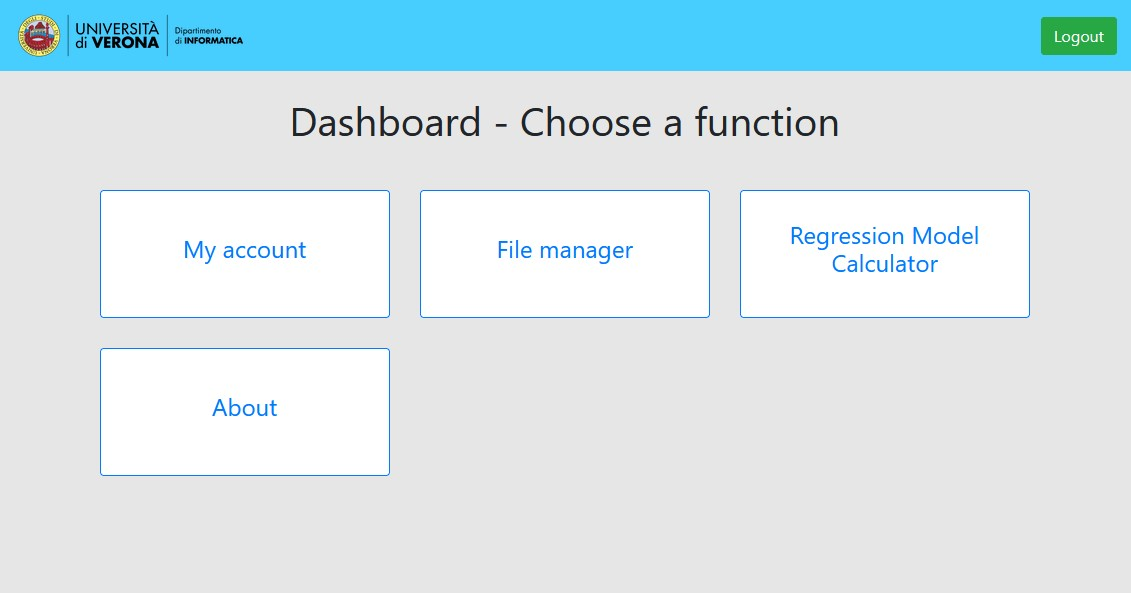
\includegraphics[width=0.85\linewidth]{images/chapter4-flask-daskboard.jpg}
    \caption{Pagina di Dashboard}
\end{figure}

\subsection{Gestione account}
\label{secsub:flask-funzionalità-account}
La pagina permette di cambiare email e password dell'utente connesso.
È possibile modificare solo l'email o la password o entrambi.
Viene mostrala l'email corrente, ma non la password per ragioni di sicurezza.
Quando si inseriscono dei valori si ha la possibilità di premere il tasto per aggiornare i dati.
Se viene superato il controllo del form, viene aggiornato il database e poi viene mostrato il messaggio di avvenuta modifica.
\begin{figure}[htp]
    \centering
    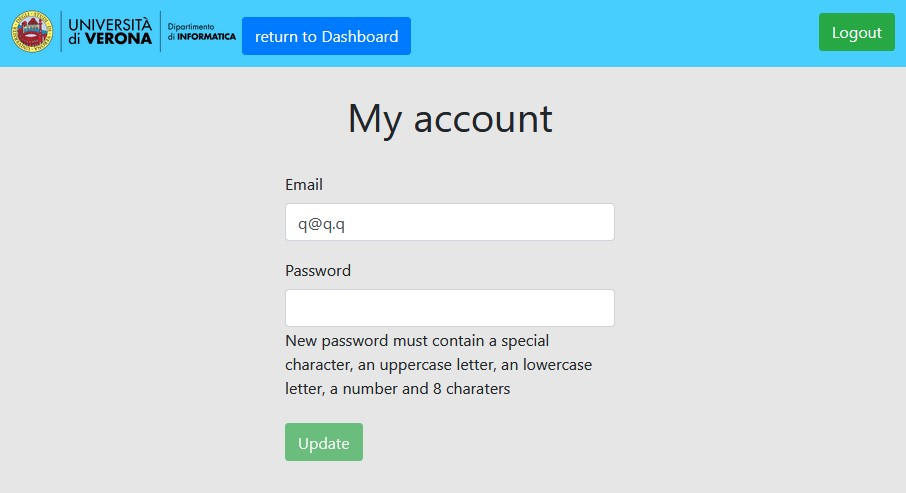
\includegraphics[width=0.85\linewidth]{images/chapter4-flask-myaccount.jpg}
    \caption{Pagina di gestione account}
\end{figure}

\newpage
\subsection{Gestione dei file}
\label{secsub:flask-funzionalità-file}
La pagina permette la gestione delle cartelle e dei file generati con la creazione dei modelli.
L'utilizzo di Javascript ha permesso di implementare la visualizzazione modificando il DOM (Document Object Model),
il quale rappresenta la pagina HTML visualizzata.
Javascript esegue delle chiamate API al server e mostra la lista delle cartelle e dei file richiesti.
Sono state implementate inoltre varie funzionalità, come la possibilità di scaricare un file singolo o l'intera cartella, 
di rinominare e di eliminare file e cartelle.
Nel download è possibile scegliere se scaricare un singolo file oppure una cartella in formato zip.
Le funzioni rinomina e cancella mostrano entrambe una finestra per confermare l'azione che si sta eseguendo.
\begin{figure}[htp]
    \centering
    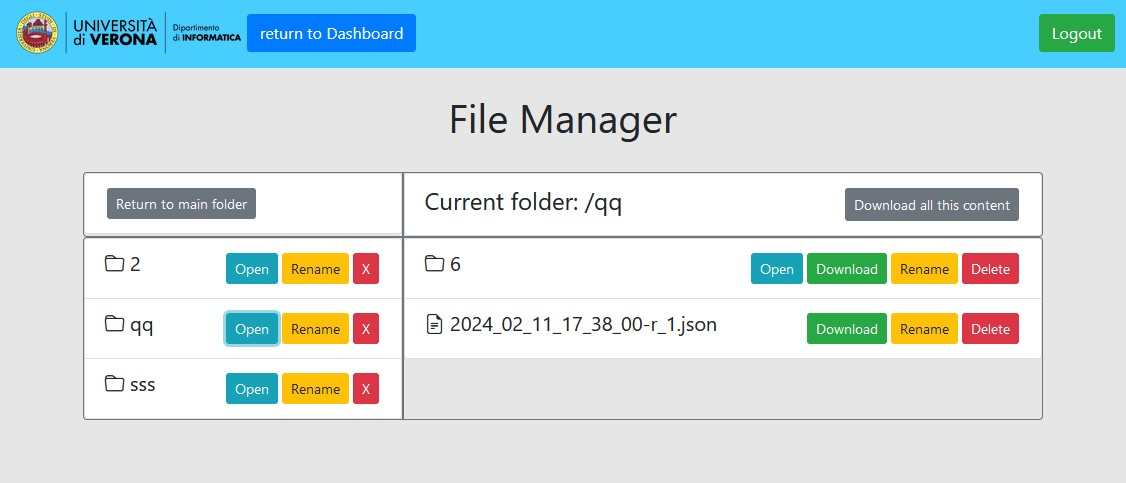
\includegraphics[width=0.85\linewidth]{images/chapter4-flask-file_manager.jpg}
    \caption{Pagina di gestione file}
\end{figure}

\subsection{Creazione dei modelli}
\label{secsub:flask-funzionalità-regressione}
La pagina permette la creazione dei modelli di regressione lineare.
La pagina è stata strutturata in due colonne.
In quella di sinistra è presente il form per l'inserimento dei dati e dei file, 
mentre quella a destra mostra le fasi di elaborazione.
Il form è strutturato nel seguente modo:
\begin{itemize}
	\item \textbf{Model Output Directory}: permette di creare o scegliere una cartella in cui il server salverà
	i file dopo l'esecuzione dello script. La cartella è accessibile tramite la pagina di gestione file.
	\item \textbf{Model Result Name}: permette di specificare quale sarà il nome dei file ottenuti dallo script.
	È un valore opzionale perché in automatico vengono messi sempre come prefisso la data e l'ora corrente.
	\item \textbf{Model Input}: permette di caricare un file in formato CSV contenente i dati storici relativi al sensore. 
	\item \textbf{Model expected output}: permette di caricare uno o più file in formato CSV 
	che rappresentano la variabile di risposta da prevedere.
	\item \textbf{Windows}: è un valore espresso come numero intero non negativo, che
	stabilirà quanti istanti temporali precedenti verranno considerati durante il
	processo di creazione del modello.
	\item \textbf{Test}: permette di scegliere se eseguire il test del modello. 
	In caso affermativo, i dati verranno divisi in addestramento (80\%) e test (20\%) per la verifica della precisione.
\end{itemize}
Una volta terminata la compilazione del form, se i campi necessari sono stati completati viene abilitato il pulsante per inviare i dati.
Se premuto, i dati vengono inviati e viene verificato se soddisfano i requisiti.
Se l'esito è positivo, nella parte destra viene mostrata la fase 1, che dà esito positivo con OK oppure segna ERROR con indicati i campi errati.
Dopo l'esito positivo viene avviata la fase 2 in cui il codice Javascript chiama una API del server per avviare
lo script che esegue la creazione dei modelli. L'utente vedrà un timer e una barra di caricamento nell'attesa.
Al termine dello script il timer si ferma e viene mostrata la fase 3 in cui sono presenti i risultati dell'elaborazione.
Viene anche mostrato un pulsante per andare al gestore dei file.\newline
L'esecuzione dello script può richiedere tempo: per risolvere il problema, l'avvio del calcolo è stato fatto tramite
Javascript in modo che la richiesta non vada in timeout, ma aspetti il termine della computazione.
\begin{figure}[htp]
    \centering
    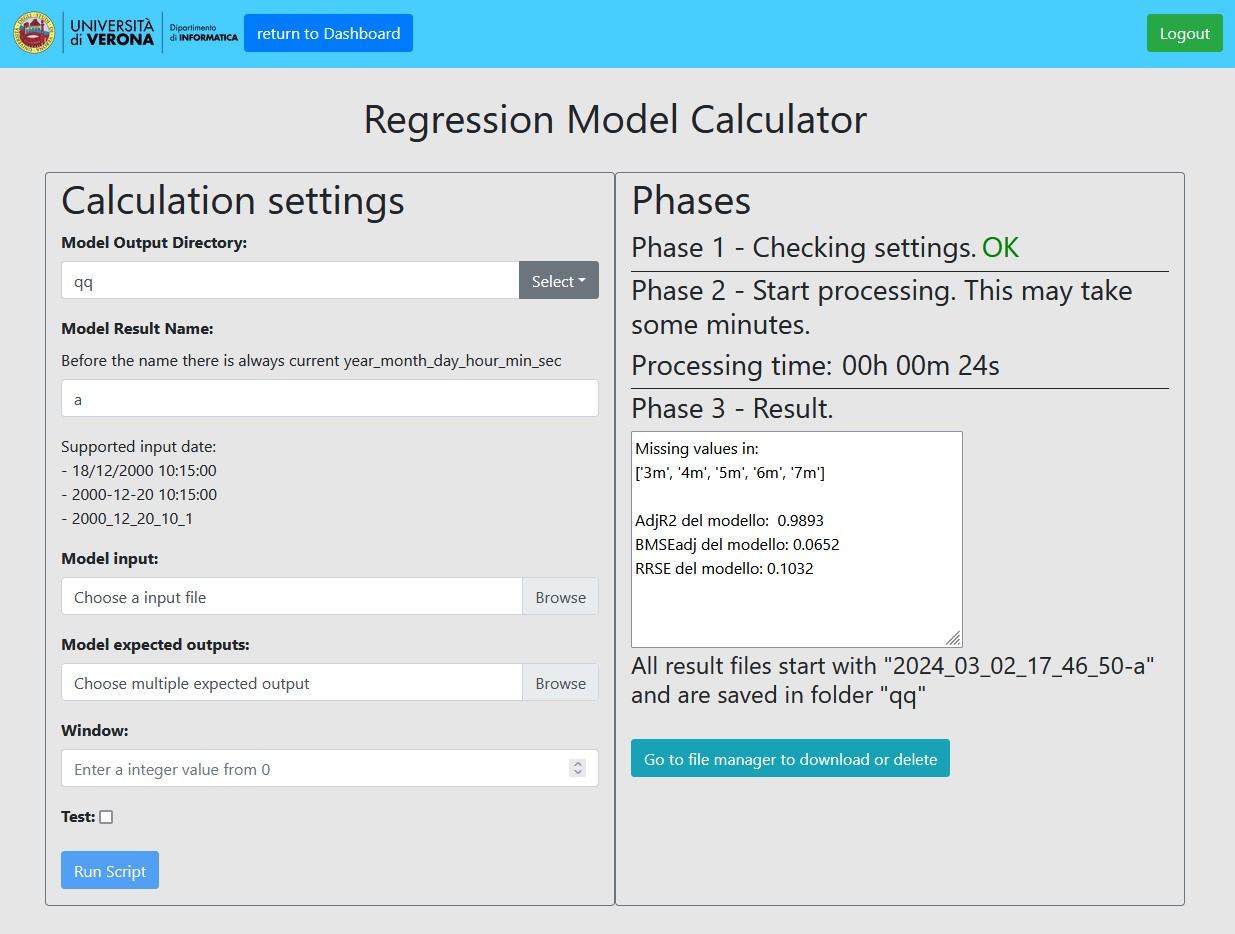
\includegraphics[width=0.7\linewidth]{images/chapter4-flask-regression.jpg}
    \caption{Pagina del calcolo del modello di regressione}
\end{figure}

\newpage
\subsection{Chi siamo}
\label{secsub:flask-funzionalità-about}
In questa pagina sono presenti l'elenco di chi ha collaborato al progetto e le immagini dei volantini presenti alla fiera.
\begin{figure}[htp]
    \centering
    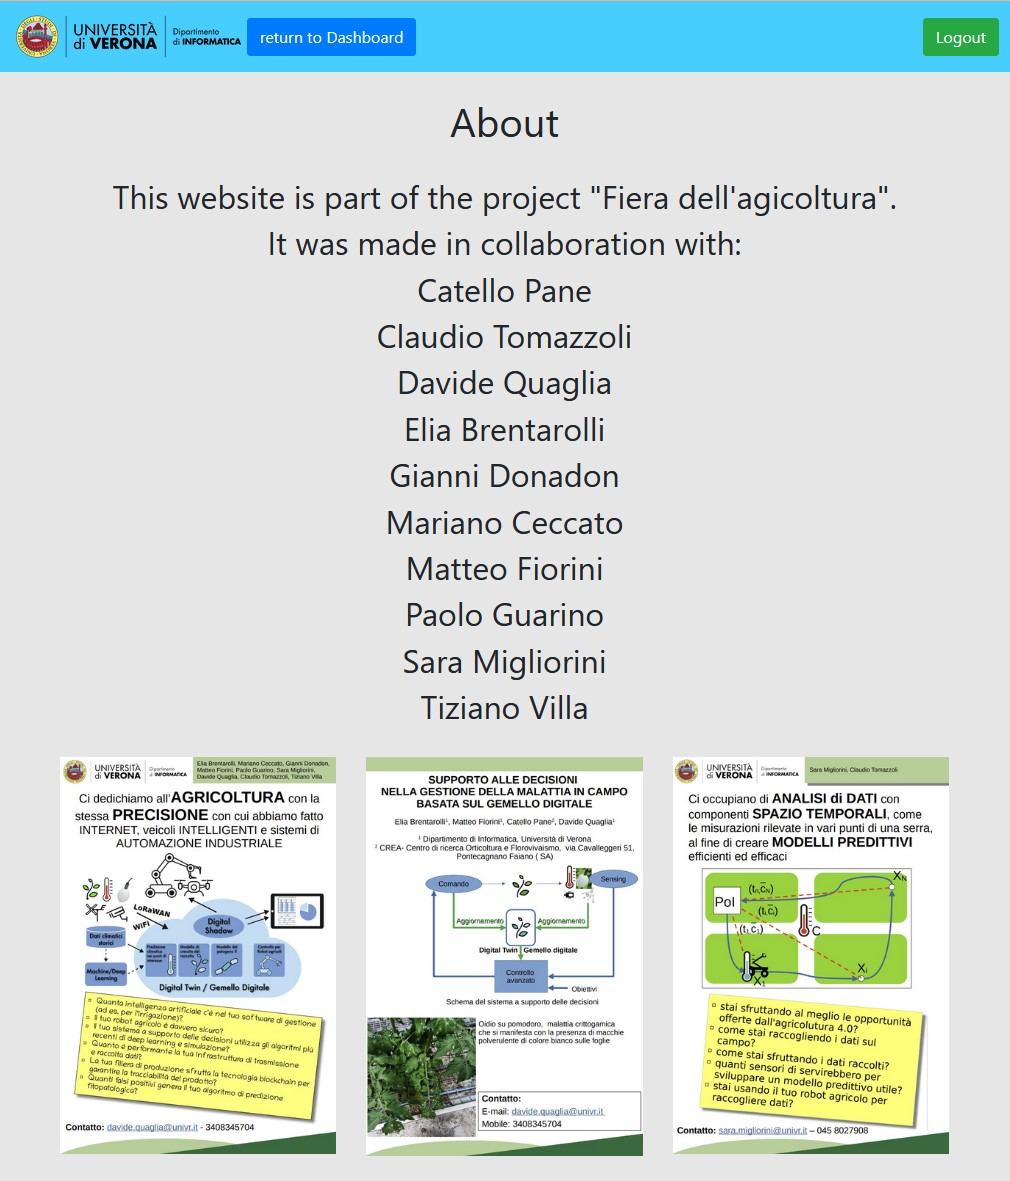
\includegraphics[width=0.7\linewidth]{images/chapter4-flask-about.jpg}
    \caption{Pagina di chi siamo}
\end{figure}

\section{Deployment}
\label{sec:flask-produzione}
Finora il progetto è sempre stato avviato in modalità sviluppo (development).
Tuttavia il server WSGI interno a Flask non è pensato per la messa in esercizio del web server 
quindi si deve usare un altro programma.
Il server WSGI di Flask è sia un server WSGI che un server HTTP, 
quindi si devono trovare due server corrispondenti per il deployment.
Nella documentazione ufficiale vengono elencati alcuni server che si possono usare \cite{flask-doc-deploying}.
Nel progetto è stato usato Gunicorn come server WSGI perché funziona interamente su Python ed è semplice da configurare.
Il server WSGI (Web Server Gateway Interface) è un protocollo di trasmissione che stabilisce e descrive comunicazioni 
ed interazioni tra server ed applicazioni web scritte nel linguaggio Python.
È quindi l'interfaccia standard del web service per la programmazione in Python.
Questo protocollo specifica come i server devono farsi carico delle richieste provenienti dai browser/client e
come devono inoltrare le informazioni richieste alle relative applicazioni, 
oltre a come utilizzare le informazioni di cui si sono fatti carico e come rispondere.
Perciò Gunicorn è il server che si occuperà di eseguire l'applicazione Flask e 
di convertire le richieste HTTP per l'ambiente WSGI e le risposte WSGI in risposte HTTP.
Di questo server si spiegheranno l'installazione e la configurazione.
Manca però il server HTTP che gestisce le richieste e le risposte HTTP.
Nel nostro caso è stato usato NGINX dato che era già presente nella macchina, 
quindi si spiegherà la configurazione necessaria.
Infine si deve impostare Gunicorn per l'avvio automatico tramite Supervisor.

\subsection{Gunicorn}
\label{secsub:flask-produzione-gunicorn}
Di seguito vengono spiegati i comandi usati nel progetto (per i dettagli vedere la documentazione ufficiale \cite{flask-doc-deploying-gunicorn}).
Nello stesso ambiente virtuale in cui si è installato Flask si può installare anche Gunicorn.
Quindi una volta avviato l'ambiente si può procedere con il seguente comando:
\begin{lstlisting}[language=python]
	pip install gunicorn
\end{lstlisting}
Per eseguire il progetto Flask in modalità produzione si deve eseguire il file run\_flask.py tramite Gunicorn.
Il file run\_flask.py è quello commentato nella spiegazione del flusso base \ref{secsub:flask-creazione-basi}
ed è rimasto invariato nelle modifiche del progetto.
Il comando per eseguire tramite Gunicorn è il seguente:
\begin{lstlisting}[language=python]
	gunicorn -w 3 run_flask:app --timeout 0
\end{lstlisting}
I parametri che vengono passati a Gunicorn sono tre.
Il parametro "-w 3" indica quanti processi devono essere avviati per servire il web server.
In questo caso sono indicati 3 processi controllati da Gunicorn che gestiranno le richieste,
così da poter rispondere a più richieste in contemporanea.
Il parametro "run\_flask:app" indica lo script che deve essere eseguito 
e il nome della variabile con cui deve essere eseguito Flask.
Infine il parametro "--timeout 0" indica che i processi di Gunicorn non devono essere interrotti
se l'esecuzione richiede troppo tempo.
L'impostazione a 0, cioè tempo infinito, è stata necessaria dato che l'esecuzione dello script 
di calcolo della regressione può richiedere svariati minuti e il timeout di default è troppo breve.\newline
Per non passare tutti i parametri è possibile creare una configurazione per Gunicorn.
Nel progetto è stata messa nel file gunicorn-config.py ed è la seguente:
\begin{lstlisting}[language=bash]
	bind = '127.0.0.1:8001'
	workers = 3
	timeout = 0
\end{lstlisting}
Oltre ai due parametri precedenti è stato aggiunto quello di bind.
Questo parametro è servito per indicare l'host e su quale porta Gunicorn deve essere in ascolto per le richieste.
Nel progetto si è dovuto specificare che l'host di ascolto è solo locale e che la porta da usare è la numero 8000, 
perché la porta di default 8080 era occupata da un altro servizio.\newline
Per eseguire Gunicorn con il file di configurazione, il comando è:
\begin{lstlisting}[language=python]
	gunicorn -c ./deploy/gunicorn-config.py run_flask:app
\end{lstlisting}
Il server WSGI è stato quindi avviato correttamente.
Per terminarlo basta premere CTRL + C.

\subsection{NGINX}
\label{secsub:flask-produzione-nginx}
Nella macchina su cui si doveva fare l'installazione era già presente NGINX, 
quindi si può fare riferimento alla documentazione ufficiale per l'installazione e i dettagli \cite{flask-doc-deploying-nginx}.
Il file di configurazione per il nostro server web è stato creato nel file nginx-web-server-flask 
(si noti che non ha un'estensione).
La configurazione è la seguente:
\begin{lstlisting}[language=python]
	server {
		listen 8000 ssl;
		server_name mydomain.it;
	
		client_max_body_size 100M;
		
		ssl_certificate /etc/letsencrypt/live/mydomain.it/fullchain.pem;
		ssl_certificate_key /etc/letsencrypt/live/mydomain.it/privkey.pem;
		
		error_page 497 301 =307 https://$server_name:$server_port$request_uri;
	
		location /static {
			alias /path_to_folder/flaskr/static;	
		}
	
		location / {
			proxy_pass http://localhost:8001;
			include /etc/nginx/proxy_params;
			proxy_redirect off;
		}
	
	}
\end{lstlisting}
Nella prima riga viene specificata la porta in ascolto, la 8000, 
e che le richieste devono essere gestite con la sicurezza SSL/TLS.
Poi si indica qual è il nome del dominio del server.
Si specifica la dimensione massima del body contenuto nelle richieste,
che viene impostata a 100 MB dato che è più che sufficiente per le nostre esigenze.
Poi vengono indicati i due path necessari per l'SSL. 
A differenza di Mosquitto qui viene usato il path di riferimento fornito da Certbot, perché
NGINX viene eseguito come utente root quindi non ha problemi ad accedere ai file.
La riga successiva serve per fare il reindirizzamento delle richieste dal protocollo HTTP a HTTPS.
In questo modo si usa sempre una connessione sicura quando si fanno le richieste.
Poi si specificano due locazioni.
La prima serve per fornire i file statici dell'applicazione Flask, 
che vengono richiesti sempre con la prima parte dell'URL formata da /static.
Deve essere specificato il path assoluto della cartella dei file statici.
È anche per questo motivo che sono stati mantenuti tutti i file statici all'interno della cartella static di default,
rendendo accessibile alle richieste dirette solo quella cartella.
La seconda locazione serve invece per girare la richiesta HTTP al server WSGI Gunicorn 
che eseguirà l'applicazione.
La richiesta viene girata tramite il proxy al processo Gunicorn che viene eseguito in locale alla porta 8001.\newline
Una volta creata, la configurazione deve essere spostata nel path delle configurazioni di NGINX, che è il seguente 
(si deve essere root per eseguire questa azione):
\begin{lstlisting}[language=textnonum]
    /etc/nginx/sites-enabled/
\end{lstlisting}
Dopo la copia della configurazione si deve riavviare NGINX con il seguente comando:
\begin{lstlisting}[language=bash]
    sudo systemctl restart nginx
\end{lstlisting}
A questo punto l'applicazione Flask è raggiungibile al dominio indicato alla porta 8000.

\subsection{Avvio automatico di Gunicorn}
\label{secsub:flask-produzione-automatico}
Come ultimo step si deve impostare l'avvio automatico per Gunicorn, 
mentre per NGINX non serve fare nulla perché viene gestito come servizio con systemctl.
Per configurare l'avvio automatico di Gunicorn viene sempre usato Supervisor, visto precedentemente \ref{sec:client-supervisor}.
Viene riportato il file di configurazione:
\begin{lstlisting}[language=bash]
    [program:web-server-flask]
	directory=/home/utente/web-server-flask
	command=/home/utente/web-server-flask/venv/bin/gunicorn -c ./deploy/gunicorn-config.py run_flask:app
	user=utente
	autostart=true
	autorestart=true
	stopasgroup=true
	killasgroup=true
	stderr_logfile=/home/utente/web-server-flask/log/gunicorn/flaskblog.err.log
	stdout_logfile=/home/utente/web-server-flask/log/gunicorn/flaskblog.out.log
\end{lstlisting}
La configurazione segue la spiegazione fornita precedentemente \ref{subsec:client-supervisor-configurazione}.
La cosa più rilevante è il comando che viene passato.
La prima parte indica l'intero path dell'ambiente virtuale in cui è installato Gunicorn. 
Si è dovuto specificare il suo path all'interno dell'ambiente virtuale perché Supervisor non avvia prima l'ambiente virtuale.\newline
Poi si procede con lo spostamento della configurazione \hyperlink{lst:client-supervisor-path}{nella cartella delle configurazioni di Supervisor}.
Infine si eseguono il comando di rilettura configurazione \ref{subsubsec:client-supervisor-rilettura} 
e aggiornamento configurazione \ref{subsubsec:client-supervisor-aggiornamento} per aggiungere
Gunicorn come processo automatico.\newline
Si è quindi terminato tutto il necessario per il deployment. 
Quando la macchina viene riavviata, l'interfaccia web ritorna disponibile. 
